\clearpage
\section{Methodology}

This methodology follows established approaches in stock market prediction using deep
learning models, drawing from previous research in the 
field~\parencite{parmar2018stock, nabipour2020DeepLearning,
chang2024StockPrediction,agrawal2022StockPrediction, shaban2024SMPDL}. 

We present here the step-by-step process undertaken to build, train, and evaluate deep
learning models for \emph{WDAY stock price prediction}, ensuring that each methodological
decision is justified based on prior studies or logical reasoning.

\subsection{Data Collection}

Stock market prediction research has demonstrated that historical price trends, combined 
with technical indicators, improve forecasting accuracy~\parencite{guo2024LSTMStock,
agrawal2022StockPrediction,balasubramanian2023SystematicSurvey,phuoc2024StockPrediction}. 

The study leverages historical stock price data for Workday Inc. (WDAY), obtained from the
Alpha Vantage API. This dataset includes daily open, high, low, close, and volume prices. In
addition, the study incorporates multiple technical indicators, including 
\acrshort{macd}, \acrshort{rsi}, \acrshort{sma}, \acrshort{bb}, and \acrshort{ema}, to
enhance predictive accuracy~\parencite{parmar2018stock, nabipour2020DeepLearning,
guo2024LSTMStock}. 

Additionally, this study will incorporate \acrshort{wma}, \acrshort{mom}, 
\acrshort{obv}, \acrshort{atr} to further evaluate their contribution to improving stock
price forecasting~\parencite{shaban2024SMPDL, phuoc2024StockPrediction}. Other technical 
indicators may also be added at a later stage to refine the model’s performance and improve
predictive accuracy.

\emph{The dataset is collected over a 10 year period to capture long-term trends and 
fluctuations}, as recommended by previous research in financial forecasting. 
Studies suggest that a minimum of five years provides enough historical data to train deep
learning models effectively, while ten years ensures a broader view of varying 
market conditions~\parencite{shaban2024SMPDL,chang2024StockPrediction}.

A detailed overview of the dataset is available in Appendix~\ref{app:dataset}.

\subsection{Data Preprocessing}

To ensure high-quality input for the stock price prediction model, the dataset
underwent a structured preprocessing pipeline. The dataset consists of 
\emph{2,763 daily stock records from 2014 to 2024}, collected using the 
Twelve Data API with a \emph{1-day frequency}, ensuring reliable and structured
historical stock market data.

\subsubsection{Handling Missing Data}

Stock market datasets frequently exhibit missing values due to market closures, stock 
splits, or incomplete data collection. Addressing these gaps is essential, as missing data 
can negatively affect model accuracy and performance~\parencite{shaban2024SMPDL}. Common 
techniques for handling missing values include forward-fill and backward-fill methods, 
which ensure continuity by propagating the most recent available 
data~\parencite{shaban2024SMPDL}. However, in the case of our WDAY dataset, no missing 
values were detected, eliminating the need for any additional data imputation.

\subsubsection{Feature transformation}

Since stock market data is inherently \emph{time-series based}, the date column must be properly transformed 
into a \emph{datetime} format and set as the dataset's \emph{index}. This transformation is crucial for 
ensuring temporal consistency and optimizing analytical procedures. Proper datetime formatting enables 
various time-series-specific operations, such as trend identification and seasonal pattern detection, which 
are fundamental for accurate forecasting models~\parencite{chang2024StockPrediction}.

By setting the date as an index, the dataset benefits in multiple ways:
\begin{description}
    \item[Chronological Integrity] Ensures that stock prices are analyzed in the correct order,
    avoiding inconsistencies in sequential learning models like LSTM and GRU~\parencite{guo2024LSTMStock}.
    \item[Enhanced Feature Extraction] Facilitates time-based calculations such as moving averages, 
    momentum, and rolling-window statistics that provide deeper insights into stock 
    trends~\parencite{shaban2024SMPDL}.
    \item[Efficient Resampling] Enables aggregation or decomposition of data into different time 
    intervals, such as hourly, daily, or weekly periods, which can be beneficial for various prediction 
    models~\parencite{agrawal2022StockPrediction}.
\end{description} 

\subsubsection{Feature Selection Based}

Feature selection is a critical preprocessing step in stock market prediction models. Highly 
correlated features introduce redundancy, increase model complexity, and may lead to 
multicollinearity, negatively impacting predictive 
performance~\parencite{balasubramanian2023SystematicSurvey, guo2024LSTMStock}. By analyzing the
correlation matrix, we identify and remove features that exhibit excessive 
correlation, ensuring a more robust and interpretable model.

\paragraph{Correlation Matrix and Redundancy Removal}
The correlation matrix provides a quantitative measure of the relationships between different
technical indicators. If two features have a correlation coefficient \(\rho > 0.9\), they
contain almost identical information~\parencite{nabipour2020DeepLearning}. In such cases, one of
the two features can be removed to prevent redundancy.

\paragraph{Criteria for Feature Selection}
To systematically reduce feature redundancy, we follow these steps:
\begin{enumerate}
    \item Compute the correlation matrix for all numerical features in the dataset.
    \item Identify feature pairs with a correlation coefficient \(\rho > 0.9\).
    \item Retain one feature from each highly correlated pair based on domain relevance or predictive importance.
    \item Remove the redundant feature to improve model efficiency and prevent overfitting.
\end{enumerate}

\paragraph{Selected Features and Removed Features}
Based on our correlation analysis (based on the Figure~\ref{fig:app-correlation}), the 
following feature selection decisions were made (Table~\ref{tab:feature_selection}):

\begin{table}[H]
    \centering
    \caption{Feature Selection Based on Correlation Analysis}
    \label{tab:feature_selection}
    \begin{tabular}{cccc}
        \hline
        \textbf{Category} & \textbf{Kept Features} & \textbf{Removed Features} & \textbf{Reason} \\
        \hline\hline
        \textbf{Price} & Close & Open, High, Low & Highly correlated \\
        \textbf{Trend} & \acrshort{sma} & \acrshort{ema}, \acrshort{wma} & Highly correlated \\
        \textbf{Momentum} & \acrshort{macd} Histogram & \acrshort{macd} Signal & Derivative of MACD \\
        \textbf{Volatility} & \acrshort{bb} (Middle) & \acrshort{bb} (Lower / Upper) & Derived \\
        \textbf{Oscillators} & \acrshort{sso} D & \acrshort{sso} K & Redundant \\
        \hline
    \end{tabular}
\end{table}

\begin{figure}[H]%
    \centering
    \caption{Correlation Matrix For the Workday's Stock Dataset}
    \label{fig:app-correlation}
    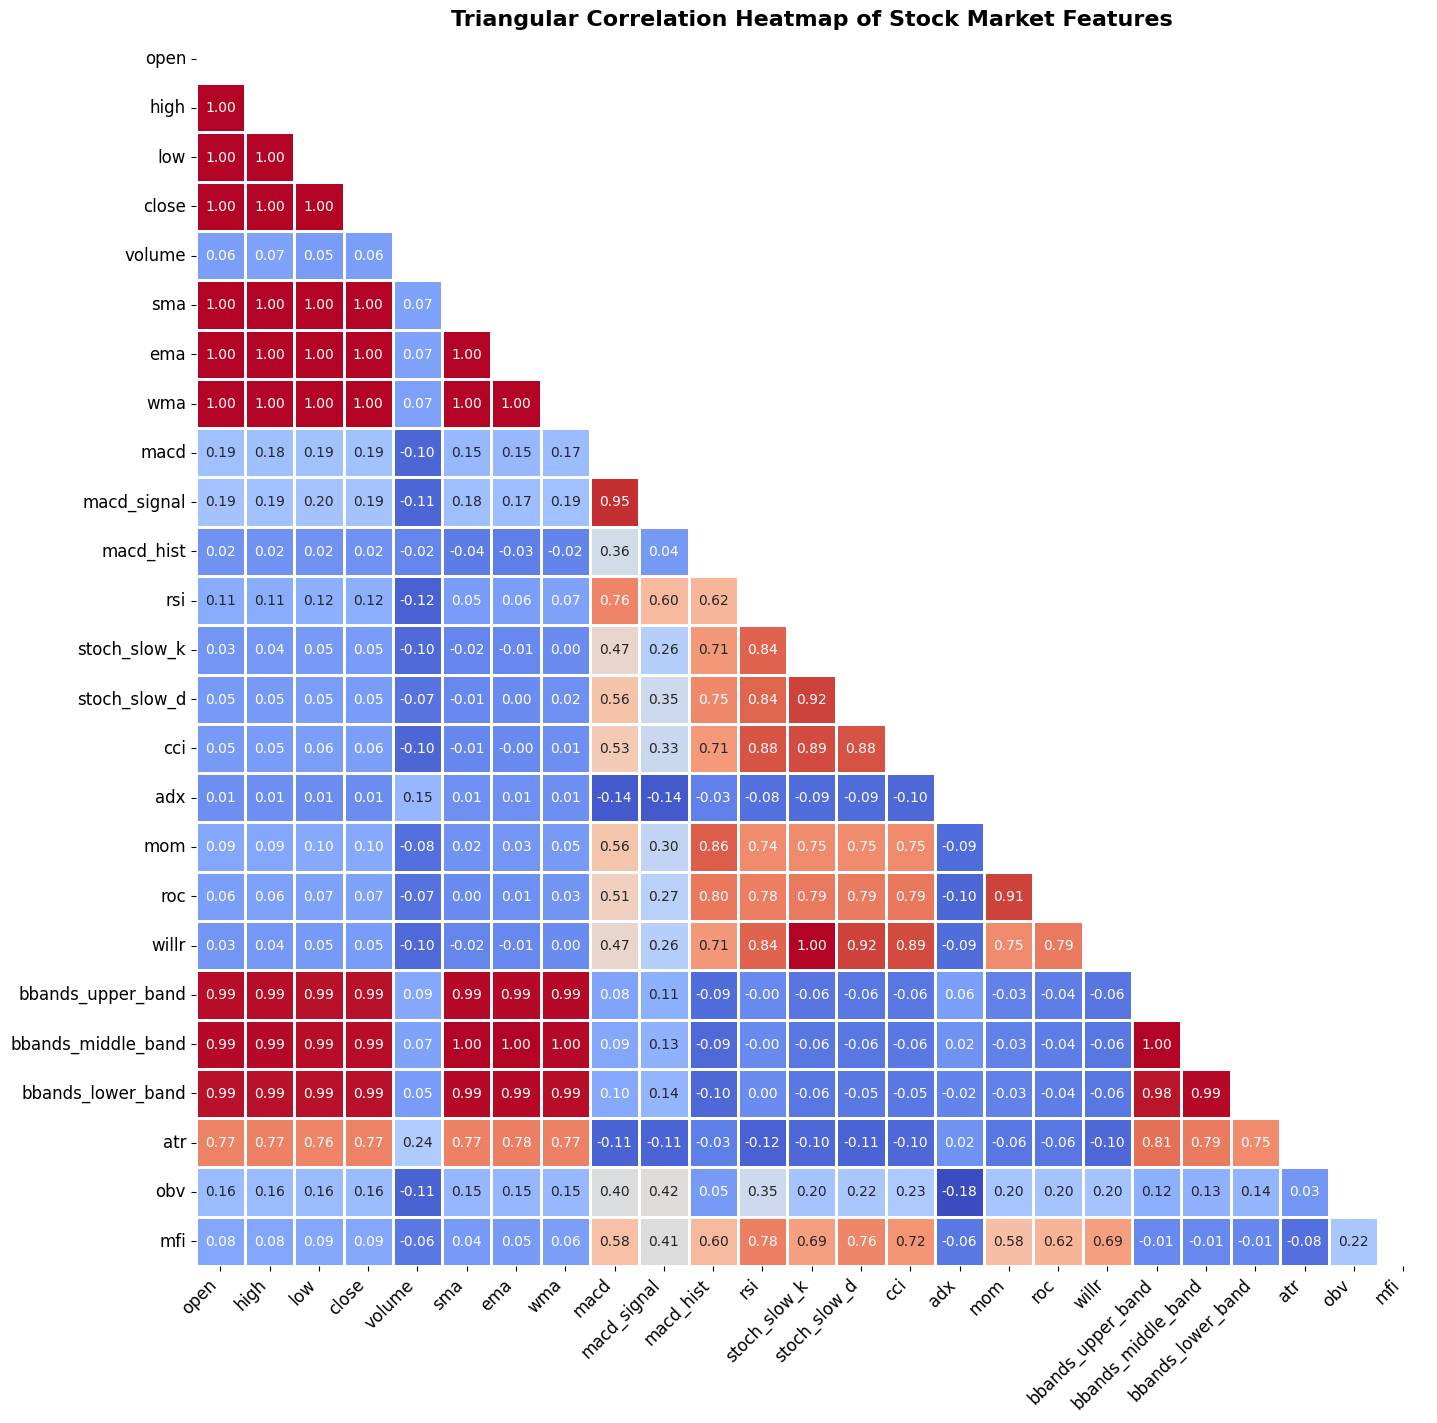
\includegraphics[width=\linewidth]{img/sections/main/correlation.png}
\end{figure}

By applying this feature selection process, we ensure that the dataset remains informative 
while avoiding unnecessary complexity. This streamlined feature set enhances model
generalization, improves training efficiency, and mitigates the risk of 
overfitting~\parencite{shaban2024SMPDL, phuoc2024StockPrediction}.

\paragraph{Summary of Feature Selection} The selected features presented in the
Table~\ref{tab:feature_selection_kept} provide 
\emph{unique information without excessive correlation}.

\begin{table}[H]
    \centering
    \caption{Feature Selected}
    \label{tab:feature_selection_kept}
    \begin{tabular}{ccp{8cm}}
        \hline
        \textbf{Category} & \textbf{Feature} & \textbf{Justification} \\
        \hline\hline
        Target & Close Price & Target variable for stock prediction. \\
        Volume & Volume & Measures market activity and confirms trends. \\
        Trend  & \acrshort{sma} & Tracks long-term price trends.\\
        Momentum & \acrshort{macd} Histogram & Captures momentum. \\
        Volatility & \acrshort{bb} Middle & Represents volatility without 
        redundant Upper/Lower bands. \\
        Oscillators & \acrshort{sso} D & More stable than Slow K, useful for 
        overbought/oversold conditions. \\
        Trend & \acrshort{adx} & Measures trend strength but not direction. \\
        Momentum & \acrshort{rsi} & Identifies potential price reversals
        using price momentum. \\
        Volatility & \acrshort{atr} & Measures price fluctuation and risk. \\
        Volume & \acrshort{obv} & Confirms price movements using volume 
        trends. \\
        Volume & \acrshort{mfi} & Combines price and volume to detect
        overbought/oversold conditions. \\
        \hline
    \end{tabular}
\end{table}

Since the dataset contains a manageable number of features (~20-25),
dimensionality reduction techniques such as \acrfull{pca}
are not required. 

The target variable in this dataset is the Close Price, representing the final
traded price of a stock at the end of each trading period, which serves as the
primary dependent variable for forecasting future stock movements.

\subsubsection{Dataset split}

In financial forecasting, time-based dataset splitting is critical to
preserving the sequential nature of stock market data. Unlike traditional
machine learning datasets, where random splitting can be applied, time-series
data must maintain chronological integrity to reflect real-world prediction
challenges. Several studies emphasize the importance of time-aware partitioning
in stock price prediction, ensuring that past data informs future forecasts
without data leakage.

For stock price forecasting, the dataset is divided as described 
in Table~\ref{tab:dataset_split}.

\begin{table}[H]
    \centering
    \caption{Time-Based Dataset Splitting Strategy}
    \label{tab:dataset_split}
    \begin{tabular}{ccp{9cm}}
        \hline
        \textbf{Dataset} & \textbf{Percentage} & \textbf{Description} \\
        \hline\hline
        Training Set & 70\% & Contains the earliest stock
        price data, allowing the model to learn long-term historical patterns. \\
        Validation Set & 15\% & Consists of the data immediately following 
        the training period, used for hyperparameter tuning. \\
        Test Set & 15\% & Represents the most recent stock prices, ensuring that 
        evaluation occurs on completely unseen future data. \\
        \hline
    \end{tabular}
\end{table}

This partitioning aligns with best practices in financial machine learning, 
where an 80/20 or 70/15/15 split balances the need for a sufficiently large 
training set while keeping a meaningful test set for 
evaluation~\parencite{chang2024StockPrediction}.

\paragraph{How the Data is Split Over Time}
As shown in Equation~\ref{eq:dataset_split}, the dataset is divided into three sequential parts to maintain chronological integrity.

Let $D={X_1,X_2,\cdots,X_T}$ be the full dataset where $X_t$ represents the stock market data at time $t$. 

\begin{equation}
\label{eq:dataset_split}
    \underbrace{X_1, X_2, \dots, X_{T_{\text{train}}}}_{\text{Training Data (70\%)}} \quad
    \underbrace{X_{T_{\text{train}}+1}, \dots, X_{T_{\text{val}}}}_{\text{Validation Data (15\%)}} \quad
    \underbrace{X_{T_{\text{val}}+1}, \dots, X_T}_{\text{Test Data (15\%)}} 
\end{equation}

This strict time-based split ensures that future data is not used to train or adjust the model, maintaining realistic forecast conditions\parencite{guo2024LSTMStock}.

\subsubsection{Feature Scaling}

Feature scaling is an essential preprocessing step in deep learning models, particularly for
time-series forecasting in stock market prediction. Models such as \acrshort{lstm}, 
\acrshort{lstmgru}, and \acrshort{lstmbigru} require properly scaled inputs to ensure stable
training, faster convergence, and improved predictive accuracy. The choice of a scaling
method significantly impacts model performance, as improper scaling can lead to gradient
instability, slow learning, or biased weight updates~\cite{chang2024StockPrediction}.

For \acrshortpl{rnn} like \acrshort{lstm} and its variants, the distribution 
and \emph{range of input features must align with activation functions such as sigmoid and tanh}. Based on the literature, 
\emph{Min-Max Scaling, Z-Score Standardization, and Robust Scaling} are the most
commonly used methods, each serving a different purpose depending on the model 
architecture~\cite{balasubramanian2023SystematicSurvey}.

Table~\ref{tab:scaling_methods} presents a comparison of the most effective feature scaling techniques for LSTM-based models, highlighting their suitability and theoretical advantages.

\begin{table}[H]
    \centering
    \caption{Comparison of Feature Scaling Methods for LSTM-Based Models}
    \label{tab:scaling_methods}
    \begin{tabular}{ccp{7.5cm}}
        \hline
        \textbf{Scaling Method} & \textbf{Best for} & \textbf{Justification} \\
        \hline\hline
        Min-Max Scaling & \acrshort{lstm} & Preserves the relative magnitude of stock price 
        movements and ensures numerical stability during training. Ideal for 
        sequential models with long-term 
        dependencies~\parencite{chang2024StockPrediction}. \\
        Z-Score Standardization & \acrshort{lstmgru} & Normalizes features to have zero mean
        and unit variance, stabilizing training and improving hybrid model 
        convergence~\parencite{balasubramanian2023SystematicSurvey}. \\
        Robust Scaling & \acrshort{lstmbigru} & Handles outliers effectively, preventing 
        distortions in bidirectional recurrent networks that analyze both past and 
        future dependencies~\parencite{shaban2024SMPDL}. \\ \hline
    \end{tabular}
\end{table}

\subsection{Model Selection}

Selecting the best model for stock price prediction is a complex task that depends on
multiple factors, including data complexity, computational efficiency, and forecasting 
accuracy. \acrshortpl{rnn} have been widely used due to their ability to capture 
time-series dependencies and handle sequential stock market data 
effectively~\parencite{shaban2024SMPDL}.

Recent research suggests that hybrid models combining \acrshort{lstm} with 
\acrshort{gru} or \acrshort{bigru} provide superior performance compared to standalone
architectures. \acrshort{lstmgru} balances efficiency and predictive accuracy, while 
\acrshort{lstmbigru} achieves the highest accuracy by capturing both past and future
dependencies~\parencite{chang2024StockPrediction}. Table xx summarizes the key advantages and trade-offs of these models, based on findings from deep learning applied to financial forecasting.

\begin{table}[H]
    \centering
    \caption{Comparison of Deep Learning Models for Stock Price Prediction}
    \label{tab:stock_models}
    \begin{tabular}{cp{4cm}p{4cm}p{4cm}}
        \hline
        \textbf{Model} & \textbf{Best For} & \textbf{Pros} & \textbf{Cons} \\
        \hline
        \acrshort{lstm} & Long-sequence dependencies, fundamental analysis & Captures
        long-term dependencies effectively, reduces vanishing gradient
        issues~\parencite{shaban2024SMPDL}. & High memory consumption, slower training 
        compared to GRU~\parencite{chang2024StockPrediction}. \\
        \acrshort{gru} & Real-time predictions, medium-term forecasting & Requires 
        fewer parameters, trains faster than LSTM while maintaining similar
        accuracy~\parencite{guo2024LSTMStock}. & May lose some long-term dependencies 
        compared to LSTM. \\
        \acrshort{bigru} & Volatile stocks, capturing full sequence trends & Processes 
        data in both forward and backward directions, leading to better sequence
        learning~\parencite{shaban2024SMPDL}. & Higher computational cost due to 
        bidirectional processing. \\
        \acrshort{lstmgru} & Faster training, mid-term forecasting & 
        Combines \acrshort{lstm}'s memory retention with \acrshort{gru}’s efficiency,
        achieving strong performance with reduced training 
        time~\parencite{chang2024StockPrediction}. & May not capture as much detail as 
        \acrshort{bigru} in highly volatile markets. \\
        \acrshort{lstmbigru} & High-accuracy stock forecasting, volatile markets & 
        Captures both forward and backward dependencies, significantly improving 
        predictive accuracy in volatile stocks~\parencite{shaban2024SMPDL}. & 
        Higher computational cost compared to \acrshort{lstmgru}, requiring more 
        processing power. \\ \hline
    \end{tabular}
\end{table}

For Workday (WDAY) stock prediction, the approach will involve implementing and evaluating 
three deep learning models: \acrshort{lstm}, \acrshort{lstmgru}, and \acrshort{lstmbigru}.
These models are selected due to their ability to capture long-term dependencies, 
short-term trends, and bidirectional patterns in stock market data.

To ensure optimal performance, the process will include:
\begin{itemize}
    \item Properly scaling the input features using an appropriate scaling technique.
    \item Searching for the best hyperparameters to optimize learning rate, batch size, number of layers, and hidden units.
    \item Evaluating model performance.
\end{itemize}

\subsubsection{Understanding RNN, LSTM, and GRU}

\begin{figure}[H]
    \centering
    \caption{Comparison of RNN, LSTM, and GRU architectures,}
    \label{fig:rnn-lstm-gru}
    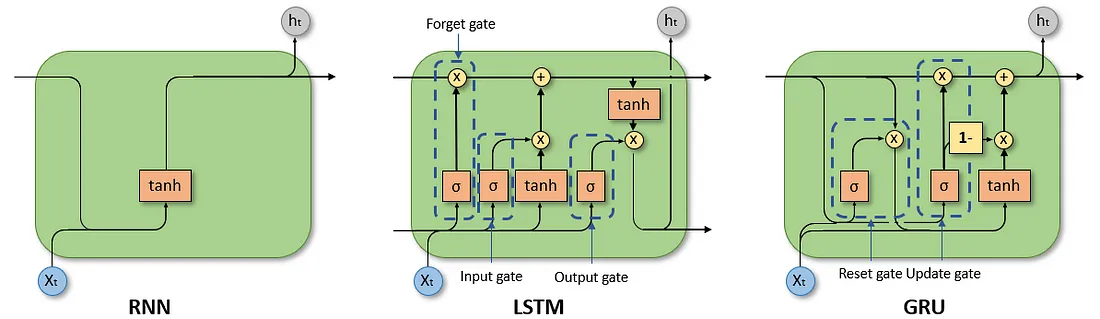
\includegraphics[width=\textwidth]{img/sections/main/rnn-lstm-gru.png}
\end{figure}

\acrfullpl{rnn} are a class of neural networks designed for sequential data processing. Unlike feedforward 
networks, \acrshortpl{rnn} incorporate loops that allow information to persist across time steps, making them well-suited 
for tasks involving sequential dependencies, such as natural language processing and time-series forecasting.

\paragraph{Architecture of RNN} An \acrshort{rnn} processes input sequences one element at a time while maintaining a
\emph{hidden state} that captures information about previous time steps. The recurrent nature of \acrshortpl{rnn} is 
represented mathematically as follows (Equation~\ref{eq:rnn_eq}):

\begin{equation}
    \label{eq:rnn_eq}
    h_t = \sigma(W_h h_{t-1} + W_x x_t + b)
\end{equation}

where:
\begin{itemize}
    \item $h_t$ is the hidden state at time step $t$
    \item $x_t$ is the input at time step $t$
    \item $W_h$ and $W_x$ are weight matrices
    \item $b$ is the bias term
    \item $\sigma$ is the activation function (commonly tanh or ReLU)
\end{itemize}

This architecture allows information to flow from past time steps to future ones~\parencite{nabipour2020DeepLearning}.

\paragraph{Limitations of RNNs}
One of the major issues with RNNs is the \emph{vanishing gradient problem}, which arises during \acrfull{bptt}. 
The gradients of earlier time steps shrink exponentially, making it difficult for the model to retain long-term 
dependencies~\parencite{parmar2018stock}.

\paragraph{LSTM Architecture} \acrfullpl{lstm} are a special type of \acrshort{rnn} designed to address the 
\emph{vanishing gradient problem}. They achieve this by introducing a \emph{memory cell} that can maintain 
information for long durations \parencite{phuoc2024StockPrediction}.

An \acrshort{lstm} unit consists of (Diagram in Figure~\ref{fig:rnn-lstm-gru}):
\begin{itemize}
\item \textbf{Forget Gate ($f_t$)} - Decides what part of the previous memory to retain.
\item \textbf{Input Gate ($i_t$)} - Regulates new information stored in the cell.
\item \textbf{Cell State ($C_t$)} - Represents the internal memory.
\item \textbf{Output Gate ($o_t$)} - Determines what information is sent to the next time step.
\end{itemize}

The computations for an \acrshort{lstm} cell are as follows:

\begin{align}
f_t &= \sigma(W_f [h_{t-1}, x_t] + b_f) \\
i_t &= \sigma(W_i [h_{t-1}, x_t] + b_i) \\
\tilde{C}t &= \tanh(W_C [h{t-1}, x_t] + b_C) \\
C_t &= f_t * C_{t-1} + i_t * \tilde{C}t \\
o_t &= \sigma(W_o [h{t-1}, x_t] + b_o) \\
h_t &= o_t * \tanh(C_t)
\end{align}

\paragraph{GRU Architecture} \acrfullpl{gru} simplify the architecture of \acrshortpl{lstm} by using only two 
gates~\parencite{chang2024StockPrediction}.

A \acrshort{gru} unit consists of:
\begin{itemize}
\item \textbf{Reset Gate ($r_t$)} - Controls how much past information should be forgotten.
\item \textbf{Update Gate ($z_t$)} - Determines the amount of new memory to retain versus past memory.
\end{itemize}

The computations for a \acrshort{gru} cell are as follows:

\begin{align}
r_t &= \sigma(W_r [h_{t-1}, x_t] + b_r) \\
z_t &= \sigma(W_z [h_{t-1}, x_t] + b_z) \\
\tilde{h}t &= \tanh(W_h [r_t * h{t-1}, x_t] + b_h) \\
h_t &= (1 - z_t) * h_{t-1} + z_t * \tilde{h}_t
\end{align}

\subsubsection{Understanding BiGRU}

\begin{figure}[H]
    \centering
    \caption{Structure of Bidirectional GRU (BiGRU): (a) GRU cell and (b) unroll BiGRU}
    \label{fig:bigru}
    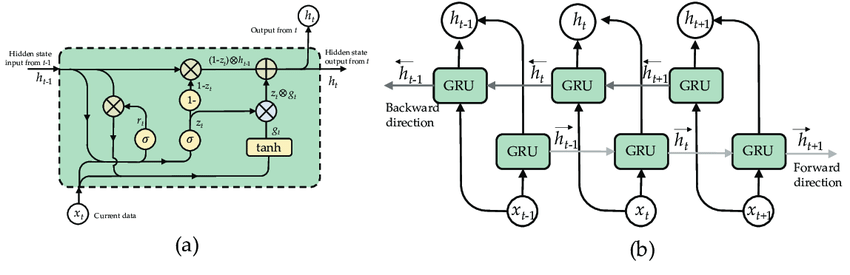
\includegraphics[width=\textwidth]{img/sections/main/bigru.png}
\end{figure}

\paragraph{BiGRU Architecture} \acrfull{bigru} is an extension of the standard \acrshort{gru} that improves sequence 
modeling by processing the input \emph{in both forward and backward directions}. This allows the network to capture 
\emph{context from both past and future time steps}, making it especially useful for tasks involving 
long-range dependencies~\parencite{shaban2024SMPDL}.

A \acrshort{bigru} processes information in two directions:
\begin{align}
\overrightarrow{h_t} &= \text{GRU}(x_t, \overrightarrow{h_{t-1}}) \\
\overleftarrow{h_t} &= \text{GRU}(x_t, \overleftarrow{h_{t+1}}) \\
h_t^{\text{BiGRU}} &= [\overrightarrow{h_t}; \overleftarrow{h_t}]
\end{align}

where:
\begin{itemize}
\item $\overrightarrow{h_t}$ is the forward GRU output.
\item $\overleftarrow{h_t}$ is the backward GRU output.
\end{itemize}

\paragraph{Advantages of BiGRU Over GRU}

\begin{itemize}
\item \emph{Captures both past and future context} at each time step.
\item \emph{Improved performance} in time-series forecasting.
\end{itemize}

\subsubsection{Understanding Hybrid Models: LSTM-GRU and LSTM-BiGRU}

Hybrid models like \acrshort{lstmgru} and \acrshort{lstmbigru} are used to leverage the strengths of
different architectures and improve the 
accuracy, efficiency, and generalization of deep learning models in sequence-based tasks. \acrshort{lstm} is excellent at 
capturing long-term dependencies due to its gating mechanisms, which prevent vanishing gradients. However, \acrshort{gru} 
is computationally more efficient and requires fewer parameters, making it a faster alternative with comparable 
performance~\parencite{phuoc2024StockPrediction}. Combining LSTM and GRU allows models to balance memory retention and computational
efficiency, effectively capturing both short-term and long-term dependencies.

\subsubsection{Hyperparameters selection}

\paragraph{Number of Neurons and Layers} The choice of hidden layers and the number of neurons per 
layer significantly impacts the model’s capacity and ability to generalize. Based on empirical 
studies~\parencite{chang2024StockPrediction, nabipour2020DeepLearning}, 
the following guidelines are recommended:

\begin{table}[H]
\centering
\caption{Recommended Neurons and Layers for LSTM Variants}
\label{table:neurons_layers}
\begin{tabular}{cccp{5cm}}
\hline
\textbf{Model Type} & \textbf{Hidden Layers} & \textbf{Neurons per Layer} & \textbf{Use Case} \\ \hline\hline
LSTM & 1-3 & 50-200 & Basic time-series forecasting \\
LSTM-GRU & 2-4 & 100-300 & Hybrid efficiency for sequence learning \\
LSTM-BiGRU & 3-5 & 150-400 & Bidirectional dependency capture \\
\hline
\end{tabular}
\end{table}

\paragraph{Hyperparameter Tuning}
Key hyperparameters and their recommended values are shown in Table~\ref{table:hyperparams}.

\begin{table}[H]
\centering
\caption{Hyperparameter Recommendations for LSTM Models}
\label{table:hyperparams}
\begin{tabular}{ccp{6.5cm}}
\hline
\textbf{Hyperparameter} & \textbf{Recommended Range} & \textbf{Description} \\ \hline\hline
Learning Rate & 0.001 - 0.0001 & Controls step size during optimization~\parencite{parmar2018stock} \\
Batch Size & 32-128 & Affects training stability and convergence \\
Optimizer & Adam, RMSprop & Commonly used for recurrent networks \\
Dropout Rate & 0.2 - 0.5 & Prevents overfitting~\parencite{agrawal2022StockPrediction} \\
Number of Epochs & 50 - 200 & Determines training iterations \\
Activation Function & Tanh, ReLU & Tanh preferred for LSTMs \\
Batch Normalization & Applied & Stabilizes training and accelerates 
convergence~\parencite{balasubramanian2023SystematicSurvey} \\
Early Stopping & Used & Prevents unnecessary computation by halting when validation loss 
stops improving~\parencite{chang2024StockPrediction} \\
\hline
\end{tabular}
\end{table}

\paragraph{Forget Gate Tuning and Avoiding Vanishing Gradients}
The forget gate in LSTM-based models regulates how much past information is discarded. Setting the 
forget bias close to 1 (e.g., $ b_f = 1 $) ensures longer 
retention~\parencite{balasubramanian2023SystematicSurvey}. Additionally, gradient 
clipping (e.g., max norm of 5) and layer normalization help prevent exploding and vanishing 
gradients~\parencite{chang2024StockPrediction}.

\paragraph{Optimal Lookback Period for Time-Series Forecasting} Selecting an appropriate number
of past days for prediction significantly affects model accuracy. General 
recommendations~\parencite{shaban2024SMPDL, phuoc2024StockPrediction} are shown in Table~\ref{table:lookback}.

\begin{table}[H]
\centering
\caption{Recommended Lookback Days for LSTM Models}
\label{table:lookback}
\begin{tabular}{cc}
\hline
\textbf{Prediction Horizon} & \textbf{Recommended Lookback Days} \\ \hline\hline
Short-term (1-5 days ahead) & 30-60 days \\
Medium-term (5-30 days ahead) & 90-180 days \\
Long-term (30+ days ahead) & 180-365 days \\\hline
\end{tabular}
\end{table}

\subsection{Performance and evaluation}

The selection of evaluation metrics is based on established research in stock market 
forecasting~\parencite{agrawal2022StockPrediction, nabipour2020DeepLearning, guo2024LSTMStock}:

\begin{description}
\item[\acrfull{rmse}] Measures the standard deviation of residuals between predicted and 
                      actual values. Lower values indicate better predictive performance.
\item[\acrfull{mae}] Represents the average absolute difference between predicted and 
                     actual stock prices.
\item[\acrfull{mse}] Highlights prediction errors with a quadratic penalty, making it 
                     sensitive to larger deviations.
\item[\acrfull{r2}] Indicates how well the model explains the variance in the data, with values 
                    closer to 1 denoting better performance.
\end{description}

\subsection{Methodology workflow}

\begin{figure}[H]
    \centering
    \caption{Workflow for Stock Market Prediction using LSTM and related models}
    \label{fig:modelwf}
    \begin{tikzpicture}[node distance=2cm]
        \node (dataset) [startstop] {Twelve Stock Market Dataset};
        \node (api) [process, below of=dataset] {\textbf{Fetch Wday Stock Prices and Indicators}};
        \node (preprocessing) [process, below of=api] {\textbf{Data Preprocessing}};
        \node (learning) [process, below of=preprocessing] {\textbf{Learning Algorithms}};
        \node (hyperparam) [process, right of=learning, xshift=3.5cm] {\textbf{Hyperparameter Tuning}};
        \node (validation) [process, below of =learning] {\textbf{Cross Validation}};
        \node (performance) [process, below of=validation] {\textbf{Performance Measures}};
        \node (comparison) [process, below of=performance] {\textbf{Comparison of Results}};
    
        \draw [arrow] (dataset.south) -- (api.north);
        \draw [arrow] (api.south) -- (preprocessing.north);
        \draw [arrow] (preprocessing.south) -- (learning.north);
        \draw [arrow] (hyperparam.west) --(learning.east);
        \draw [arrow] (learning.south) -- (validation.north);
        \draw [arrow] (validation.south) -- (performance.north);
        \draw [arrow] (performance.south) -- (comparison.north);
    \end{tikzpicture}
\end{figure}

The diagram (Figure~\ref{fig:modelwf}) presents a structured workflow for stock market prediction 
using \acrshort{lstm} and related deep learning models. The workflow is divided into key stages that
ensure a systematic approach to data processing, training, evaluation, and comparison. Below is a 
step-by-step breakdown of each component:

\begin{description}
    \item[Twelve Stock Market Dataset] The process begins with collecting stock market data from
         twelve different markets. This dataset serves as the foundation for training and evaluation
    \item[Fetch Wday Stock Prices and Indicators]  From the dataset, Workday (WDAY) stock prices 
         and technical indicators are extracted for predictive modeling.
    \item[Data Preprocessing] Raw stock price data undergoes cleaning, normalization, and 
         transformation to ensure compatibility with machine learning models.
    \item[Learning Algorithms] The \acrshort{lstm} models are trained using the processed dataset.
    \item[Hyperparameter Tuning] Hyperparameter tuning is performed in parallel to optimize
        learning rates, batch sizes, dropout rates, and activation functions for better performance.
    \item[Cross-Validation] The models are validated using cross-validation techniques to assess 
         generalization ability and reduce overfitting.     
    \item[Performance Measures] The trained models are evaluated using metrics such as 
         \acrshort{rmse}, \acrshort{mae}, \acrshort{mse}, and \acrshort{r2} to determine 
         prediction accuracy.
    \item[Comparison of Results] The final step involves comparing the performance of 
         different models and identifying the best-performing approach for stock price forecasting.
\end{description}
